% !TEX TS-program = pdflatex
% !TEX encoding = UTF-8 Unicode

% This is a simple template for a LaTeX document using the "article" class.
% See "book", "report", "letter" for other types of document.

\documentclass[12pt]{article} % use larger type; default would be 10pt

\usepackage[utf8]{inputenc} % set input encoding (not needed with XeLaTeX)
\renewcommand\familydefault{\sfdefault}
\usepackage{helvet} 


%%% Examples of Article customizations
% These packages are optional, depending whether you want the features they provide.
% See the LaTeX Companion or other references for full information.

%%% PAGE DIMENSIONS
\usepackage[a4paper,landscape,twocolumn,margin=0.5in]{geometry} % to change the page dimensions
%\geometry{a4paper} % or letterpaper (US) or a5paper or....
%\geometry{margin=0.5in} % for example, change the margins to 2 inches all round
%\geometry{twocolumn} % two columns
%\geometry{landscape} % set up the page for landscape
%   read geometry.pdf for detailed page layout information

\setlength{\columnsep}{0.5in}

\usepackage{graphicx} % support the \includegraphics command and options
\usepackage{hyperref}

% \usepackage[parfill]{parskip} % Activate to begin paragraphs with an empty line rather than an indent

%%% PACKAGES
\usepackage{booktabs} % for much better looking tables
\usepackage{array} % for better arrays (eg matrices) in maths
\usepackage{paralist} % very flexible & customisable lists (eg. enumerate/itemize, etc.)
\usepackage{verbatim} % adds environment for commenting out blocks of text & for better verbatim
\usepackage{subfig} % make it possible to include more than one captioned figure/table in a single float
% These packages are all incorporated in the memoir class to one degree or another...

%%% HEADERS & FOOTERS
\usepackage{fancyhdr} % This should be set AFTER setting up the page geometry
\pagestyle{fancy} % options: empty , plain , fancy
\renewcommand{\headrulewidth}{0pt} % customise the layout...
\lhead{}\chead{}\rhead{}
\lfoot{}\cfoot{}\rfoot{\thepage}

%%% SECTION TITLE APPEARANCE
\usepackage{sectsty}
\usepackage{titlesec}
\allsectionsfont{\sffamily\mdseries\upshape\bfseries} % (See the fntguide.pdf for font help)
% (This matches ConTeXt defaults)

%%% END Article customizations

%%% The "real" document content comes below...

\title{\large{\vspace{-5ex}\textbf{Exploration and Modelling of Planetary Interiors}}\newline\\{\textbf{\underline{Lecture 12 - Giant Planet Formation}}}\vspace{-7ex}}
\author{}
\date{} % Activate to display a given date or no date (if empty),
         % otherwise the current date is printed 

\renewcommand*\contentsname{\large\textbf{Topics covered}\vspace{-2ex}}

\bibliographystyle{apalike}
\renewcommand\refname{Background reading}

\begin{document}
\begingroup
\let\center\flushleft
\let\endcenter\endflushleft
\maketitle
\endgroup

\begingroup
\let\cleardoublepage\relax
\let\clearpage\relax
\tableofcontents
%\listoffigures
%\listoftables
\endgroup

\begin{figure}
\begin{center}
 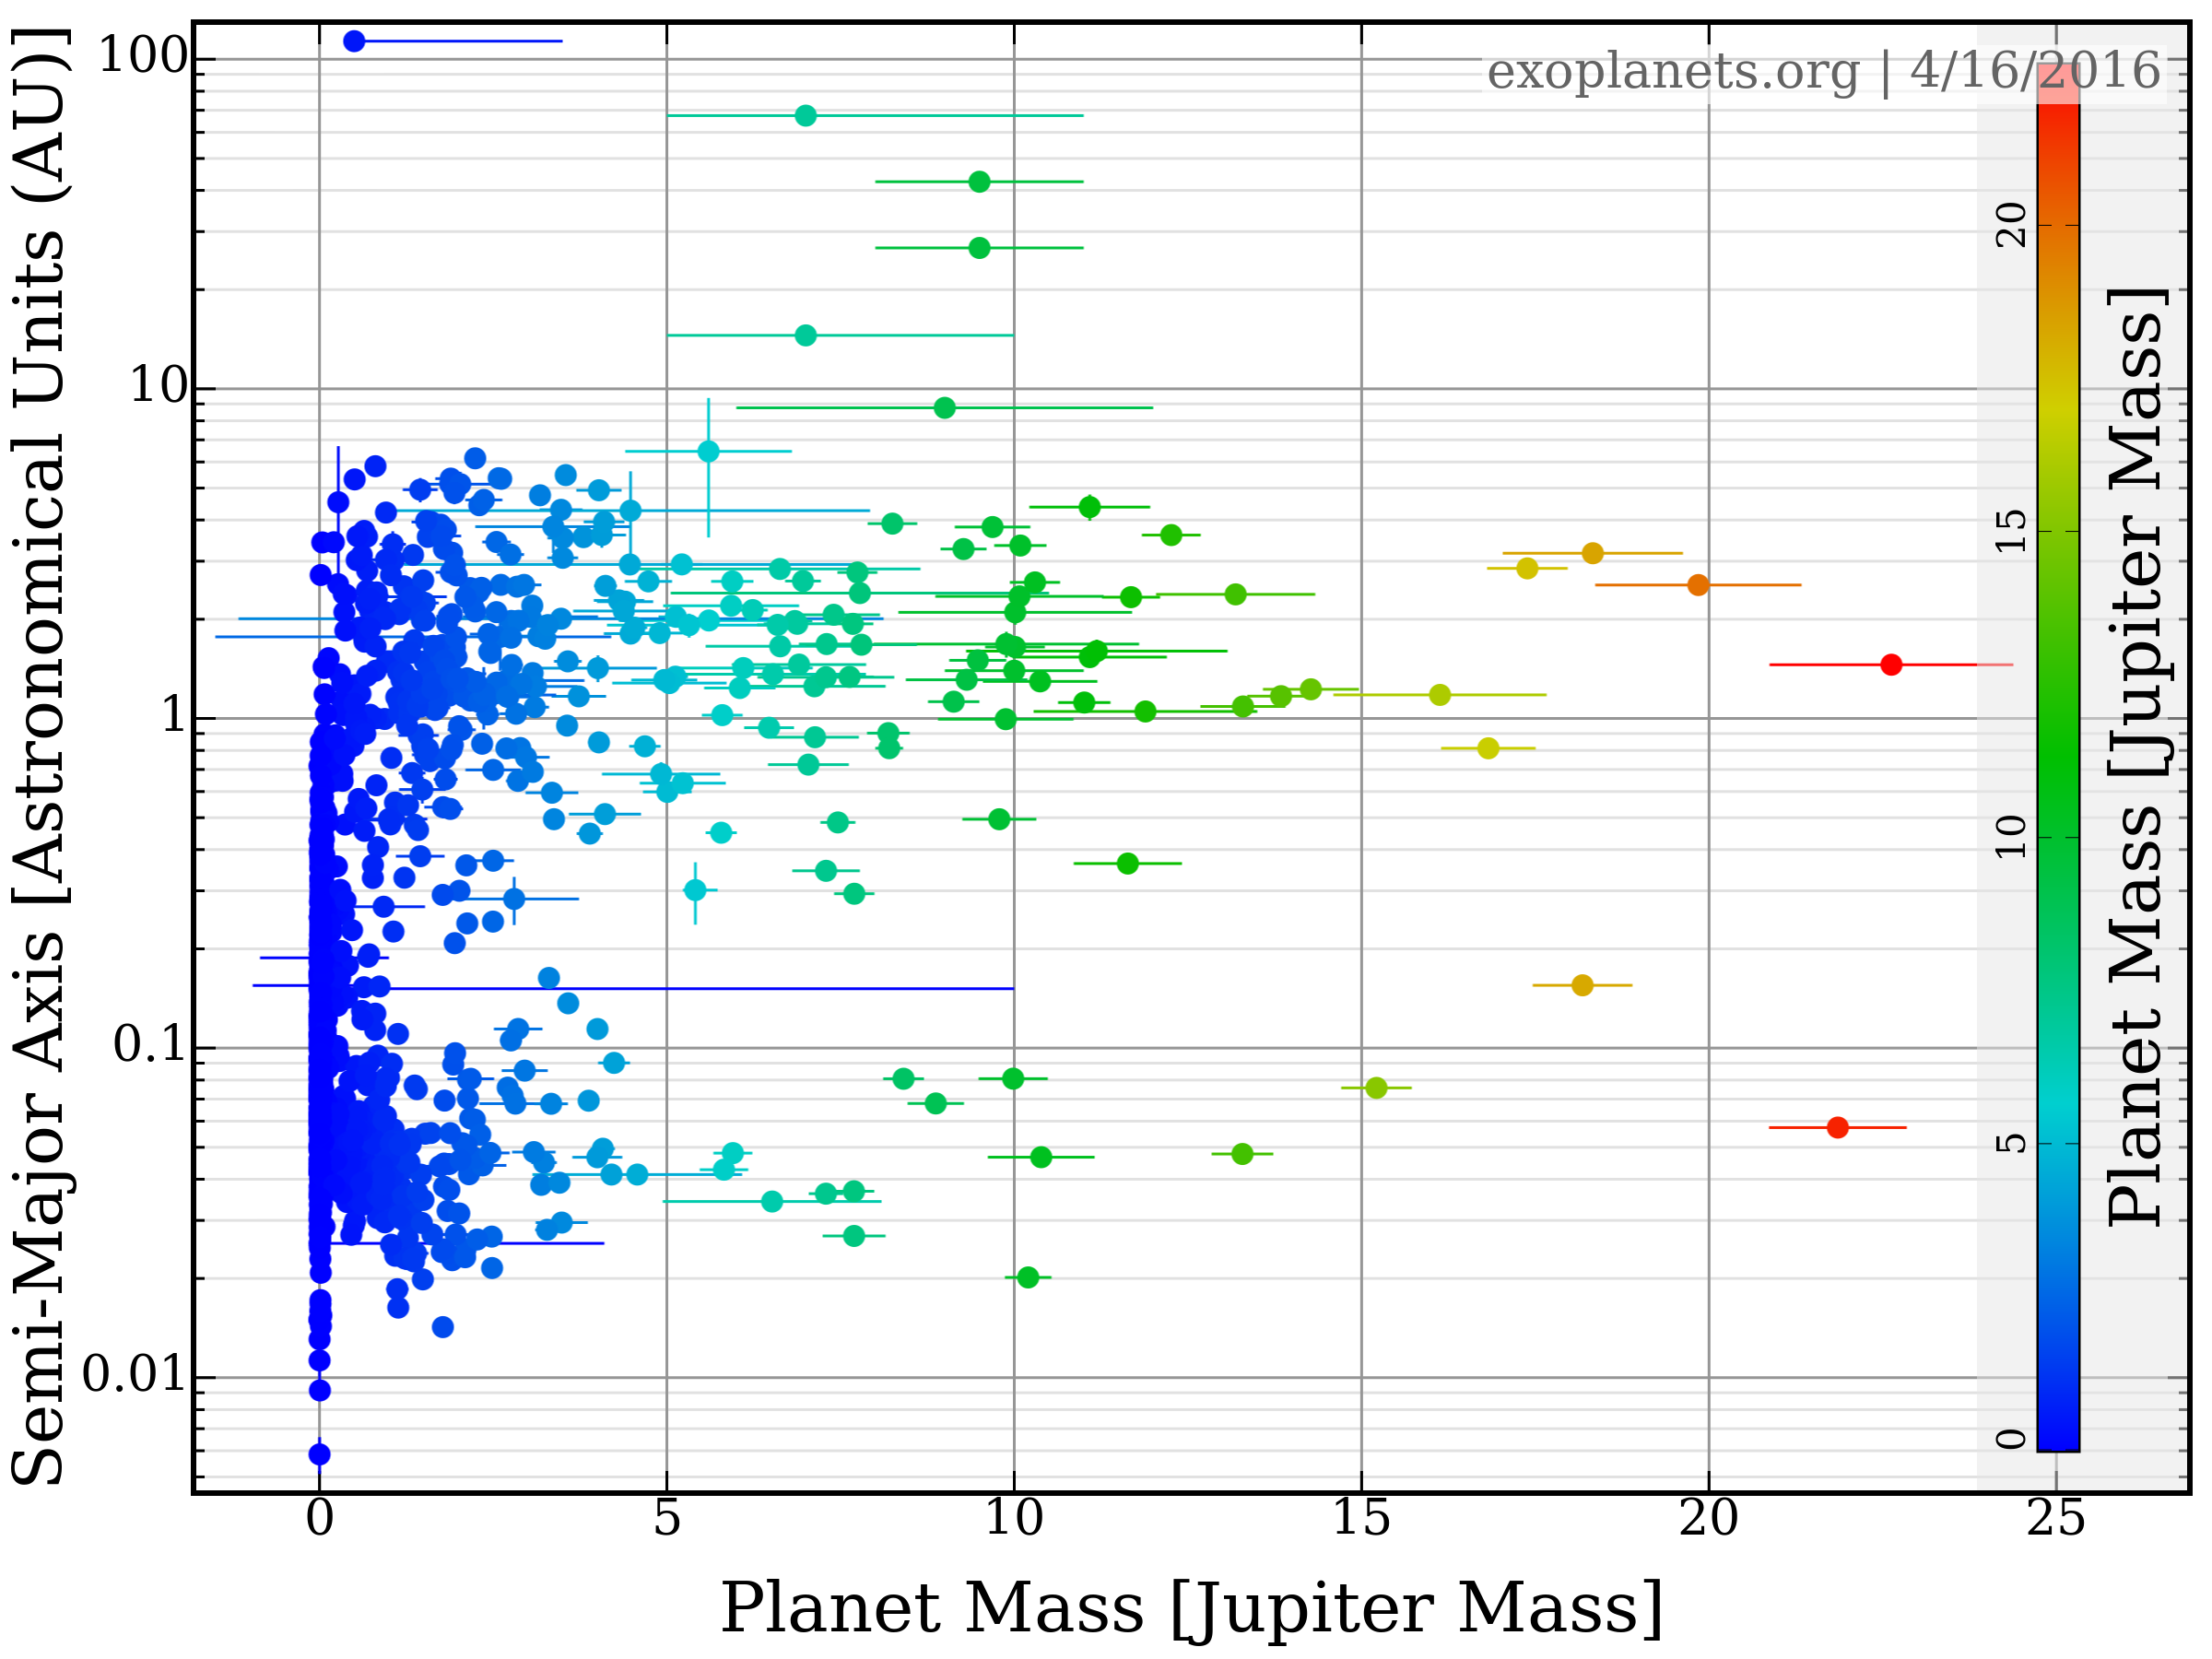
\includegraphics[width=0.5\textwidth,keepaspectratio=true]{./images/exoplanets}
 \caption{Mass/radius of exoplanets (orbit database, exoplanets.org)}
 \label{exoplanets}
\end{center}
\end{figure}


\section{Introduction}\vspace{-2ex}\titlerule[1pt]\bigskip

There are four giant planets in the solar system, Jupter, Saturn, Uranus and Neptune. The first two are called \textbf{gas giants} and the two other \textbf{ice giants}, due to their physics and their major constituting elements. Gas giants are mostly NH$_3$, CH$_4$ and H$_2$O, while ice giants are mostly H and He, and further away from the Sun.

\subsection{Exoplanetary research}\vspace{-1ex}\bigskip

It is worth mentioning here that giant planets are not limited to the solar system. Since the exoplanets search has started, many were found (Figure \ref{exoplanets}). These types were the first planets detected because of their sizes. Still now, they are the most numerous found to date. New sub-types have been defined from the exoplanet discoveries, including closely orbiting \textbf{hot Jupiters} or \textbf{hot Neptunes}. \newline\linebreak
\clearpage
\noindent The exoplanet search will certainly bring many more exotic samples to permit a better understanding of their population and their limits, especially answering better the question: ``When can we say this is a gas giant or a brown dwarf''. Two additional spectral classes of dwarf stars are completing the M dwarf (75M$_J$), they are the L dwarf (65M$_J$) and the T dwarf (30M$_J$). Some elements of observations and physics are found in \cite{Jeffries:2015:Online}, giving an introduction on electron degeneracy pressure and its impact on gas unusual state of matter (Figure \ref{gas_giants_vs_stars}) on the side of the ``cold start'' or core accretion.

\begin{figure}
\begin{center}
 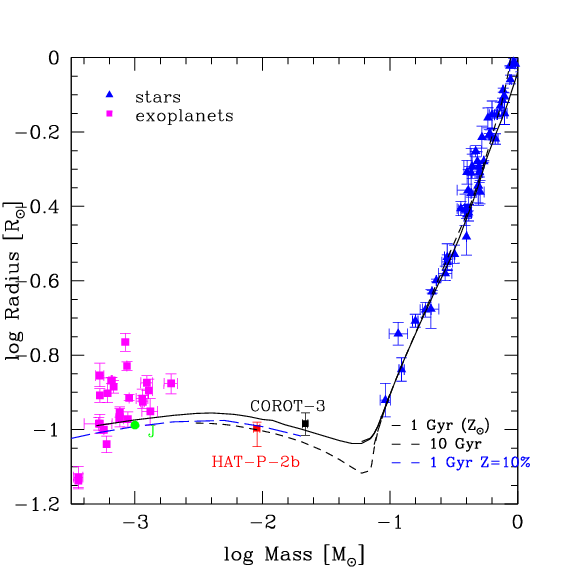
\includegraphics[width=0.45\textwidth,keepaspectratio=true]{./images/physics_stackexchange_com_questions_165283_gas_giant_six_times_more_massive}
 \caption{Mass/radius of gas giants \& stars \cite{Jeffries:2015:Online}}
 \label{gas_giants_vs_stars}
\end{center}
\end{figure}


\subsection{Schools of thought about formation}\vspace{-1ex}\bigskip

There are actually three different school of thoughts, and thus types of models that are built and tested to learn more about giant planets formation. We will investigate each one of them separately and then look at what we have learnt.

\begin{itemize}
\setlength\itemsep{0em}  
\item \textit{\textbf{Core-nucleated accretion:}} big rocks accumulated gas 
\item \textit{\textbf{Fragmentation during collapse:}} planet forms like star
\item \textit{\textbf{Giant gravitational instability in disk:}} giant protoplanets 
\end{itemize}



\section{Core-nucleated instability}\vspace{-2ex}\titlerule[1pt]\bigskip

This model assumes a fast forming planetary core. When the core accretion is well underway, the critical mass of the core generates an hydrostatic growth phase permitting gas accretion until it itself exceeds the core critical mass, when the M$_{envelope}$ = M$_{core}$ threshold is passed \cite{miguel2008core}. Eventually the disk dispersal will lead to a Kelvin-Helmholtz contraction \cite{armitage2010astrophysics}. \newline\linebreak
\clearpage

\noindent This is essentially a ``bottom-up'' phenomenon with the following steps:
\begin{itemize}
\setlength\itemsep{0em}
\item Core formation
\item Hydro-static growth
\item Run-away growth
\item End of accretion
\end{itemize}

\noindent The model proposed by \cite{pollack1996formation} is first defining planetesimal properties as a mass fraction of H$_2$O ice, rock and CHON (Carbon, Hydrogen, Oxygen and Nitrogen). Each having a density, a latent heat (+: endothermic like ice and rock \& -: exothermic like CHON) and a vaporisation temperature. It defines and simulates both the gas and the planetesimal accretion rates together. \newline\linebreak
The main assumptions in the accretion model (see Figure \ref{pollack1996}) are: 
\begin{itemize}
\setlength\itemsep{0em}
\item An isolated embryo
\item An initial phase of runaway accretion of solids
\item Small random velocities and sizes of planetesimals
\item No planetesimal migration into or out of the current feeding zone
\end{itemize}


\begin{figure}
\begin{center}
 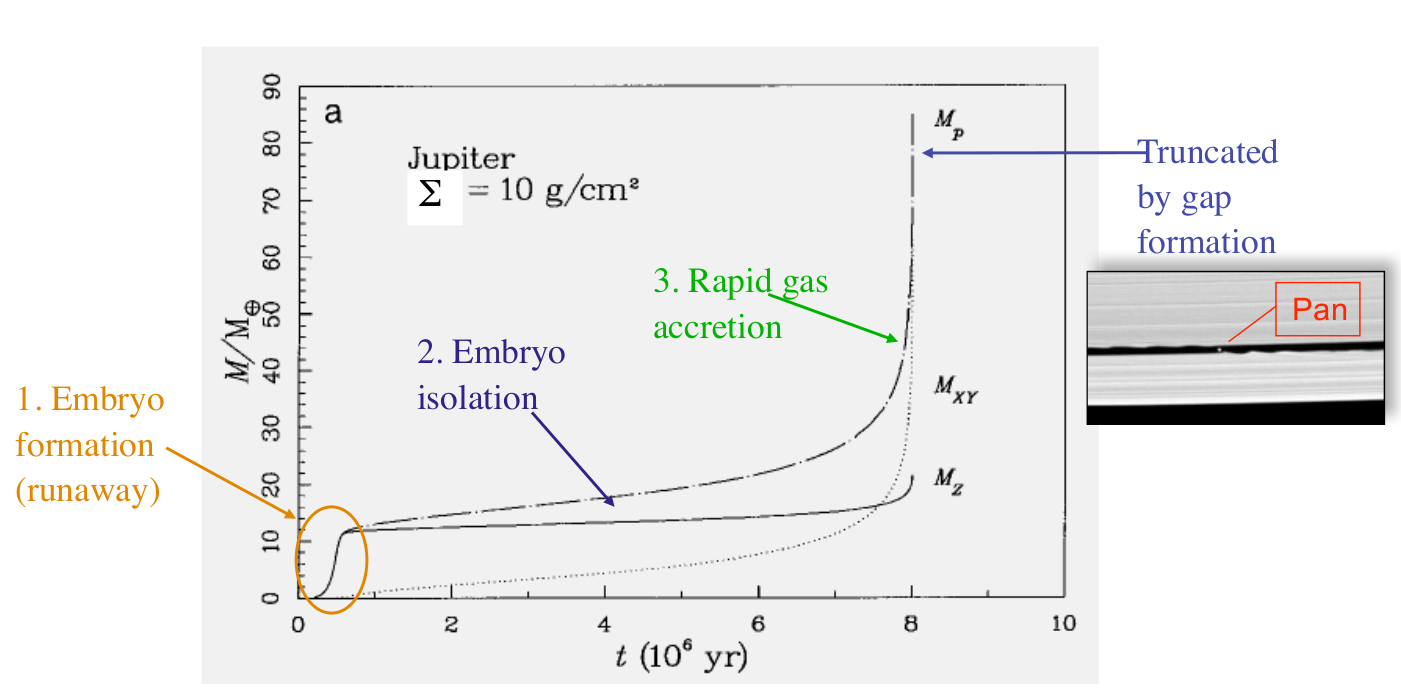
\includegraphics[width=0.5\textwidth,keepaspectratio=true]{./images/pollack1996}
 \caption{Core accretion scenario \cite{pollack1996formation}}
 \label{pollack1996}
\end{center}
\end{figure}

\noindent They defined a solar mixture of elements, X=0.74, Y=0.243, Z=0.017, M$_Z$ as the high Z-mass accreted, in opposition to M$_{XY}$ the low Z-mass accreted. They found that a variable rate of planetesimal accretion \cite{lissauer1987timescales} is vastly more responsive to recreate the four solar system giants. Their modelling results identified three phases in the giant planets formation:

\begin{itemize}
\setlength\itemsep{0em}
\item M$_Z$ $>$ Energy produced. Maximisation of its value ensues, then it is reducing to isolation mass level
\item M$_Z$ $>$ M$_{XY}$. Reduction to low constant level, M$_{XY} = 2$-$4 M_Z$ but still M$_Z$ $>$ Energy produced
\item M$_Z$ $=$ constant $=$ M$_{XY}$
\end{itemize}

\noindent Though satisfying, they found that accretion rates are too slow. They estimated that a reduction of planetesimal size along with a reduction in vertical transport would allow the acceleration of the planetary formation. This type of model is known to be slow, so that the race for mass gain to reach giant planet level is often lost due to the more rapid dissipation of the protoplanetary disk. The model from \cite{pollack1996formation} is much more efficient when the environment is characterised by high metallicity and smaller planetesimals, speeding up the core formation and the downward migration to grow the core.

\section{Fragmentation during collapse}\vspace{-2ex}\titlerule[1pt]\bigskip
Gas flow near planet. 
Detection of planet size in accretion disk from \cite{bate2003three}.\newline

\noindent Giant planet formation by gravitational fragmentation = gravitational instability = “top-down”. Uncertainties include:
\begin{itemize}
\setlength\itemsep{0em}
\item Temperature of the disk
\item Mass of the infall rate from surrounding original envelope
\item Final planet masses
\end{itemize}

\section{Giant gravitational instability in disk}\vspace{-2ex}\titlerule[1pt]\bigskip

The migration type 2 from \cite{chambers2009planetary} addresses giant planet spin and the viscous torques it generates in the accretion disk (Figure \ref{chambers2009}).\newline

\noindent While the protoplanet growth was still below giant planet mass, the type 1 migration already started to locally modify the disk structure by adding angular momentum to outward part of the disk, and reducing it in the inward part. A vaccuum effect is generated, creating the well known protoplanetary disk gap, a result of tidal interactions described. At this point onward, the planet and the viscous evolution of the disk are joined.

\begin{itemize}
\setlength\itemsep{0em}
\item Tidal interaction creates gap in disk by sourcing inner disk more
\item Inner disk shrinks
\item Angular momentum moves outward through the planet
\item Planet moves inward, may carry outer disk along (if viscosity)
\item End of inner disk, or orbit stabilization (star spin tidal interaction)
\end{itemize}

\begin{figure}
\begin{center}
 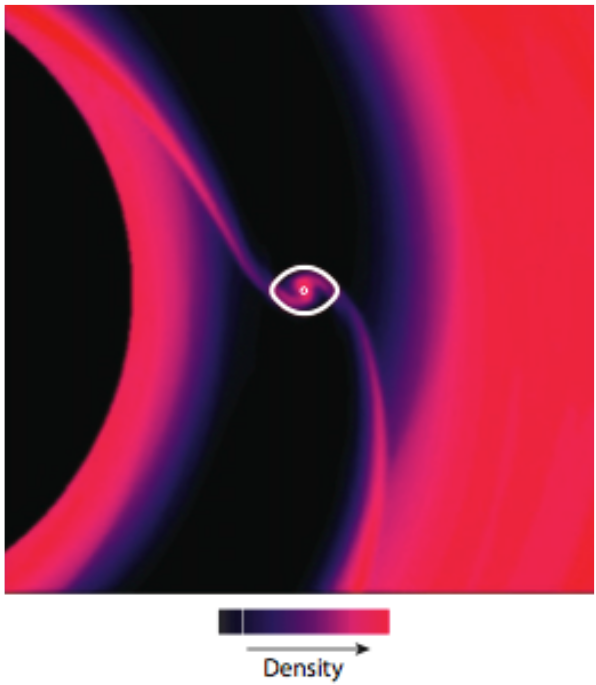
\includegraphics[width=0.5\textwidth,keepaspectratio=true]{./images/chambers2009}
 \caption{Type 2 (giant planet) migration \cite{chambers2009planetary}}
 \label{chambers2009}
\end{center}
\end{figure}


\noindent The model from \cite{lissauer2009models} is looking into the mechanisms that permit the growth from Mars mass to Jupiter mass using hydrodynamic and thermal constraints. The parameters used in this model are the disk viscosity, the surface density and planet properties. They found that when the disk has a high viscocity, accretion is higher.\newline

\noindent This model can form giant planet fast, they are formed in-situ and may migrate as seen in \cite{chambers2009planetary}. The environmental metallicity is much less important here than in \cite{pollack1996formation}.\newline
\clearpage

\begin{figure}
\begin{center}
 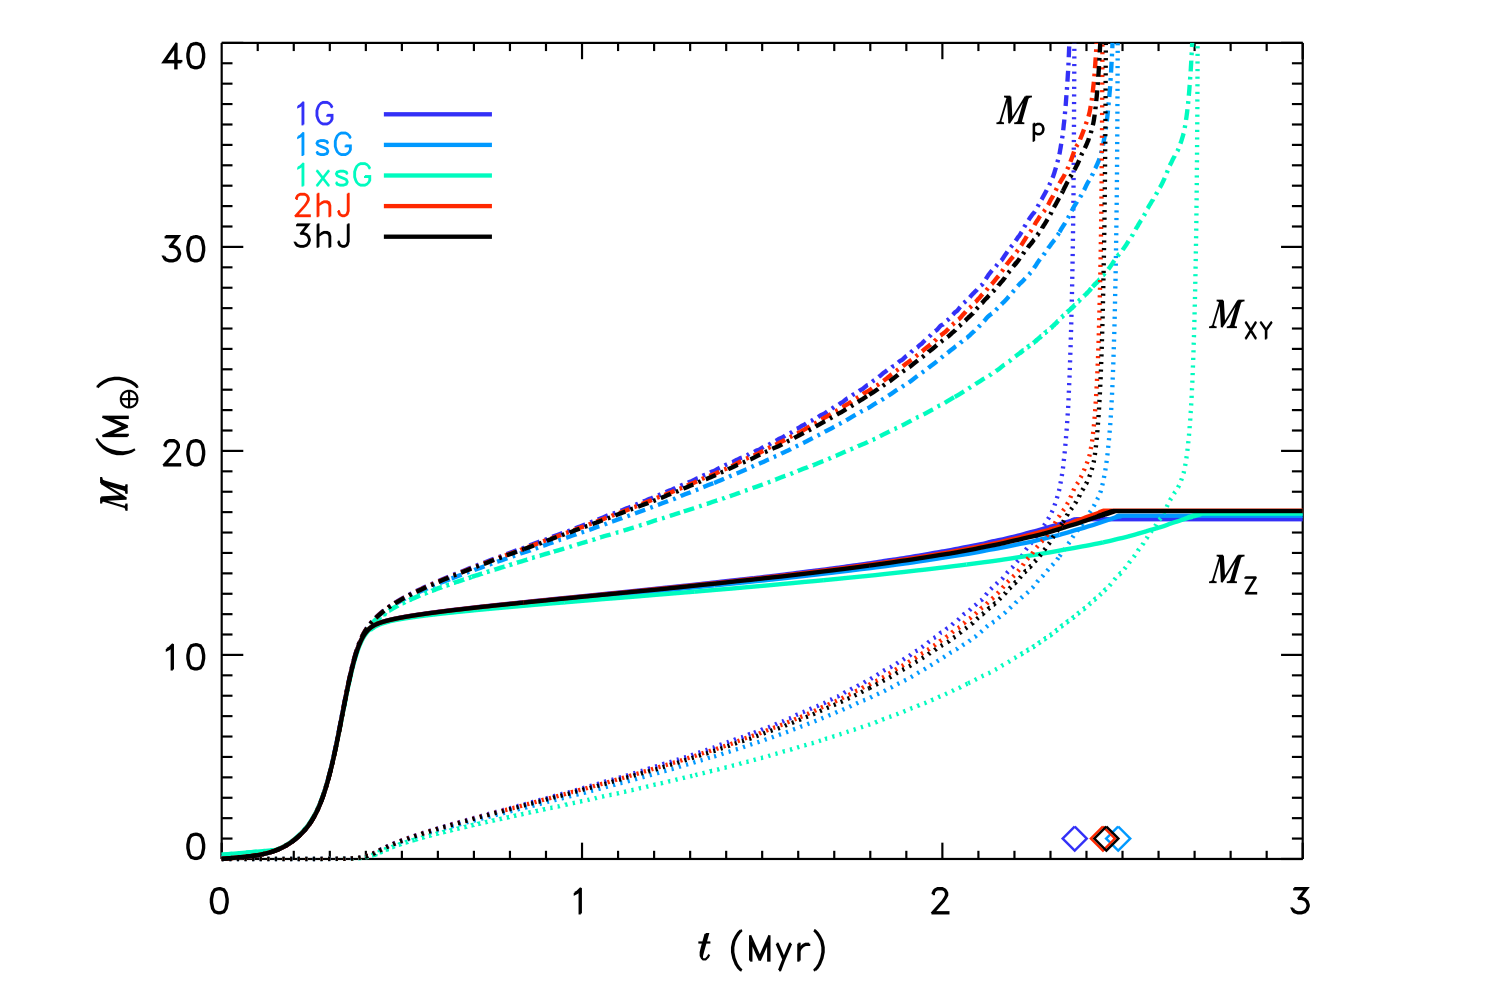
\includegraphics[width=0.5\textwidth,keepaspectratio=true]{./images/lissauer2014}
 \caption{Giant planet mass of condensibles (solid, M$_Z$), H/He (dot, M$_{XY}$) and total (dot dash, M$_P$)  \cite{lissauer2009models}}
 \label{lissauer2014}
\end{center}
\end{figure}


\noindent The Figure \ref{lissauer2014}  from \cite{lissauer2009models} is now extending the Figure \ref{pollack1996} from \cite{pollack1996formation}  with more detailed controls, due to better constraints on heat and flow dynamics. They found from 3D hydrodynamics and planetary growth simulations that: 

\begin{itemize}
\setlength\itemsep{0em}
\item  The flow of gas in the circumsolar disk limits the region occupied by the planet’s tenuous gaseous envelope to $<$
 0.25 R$_H$ (Hill sphere radii) of the planet’s center
 \item Jupiter formation: 2.5–3 Myr (with protoplanetary disk's solid surface density of 10 g.cm$^{-2}$ \& dust opacity in
protoplanet’s envelope of 2\% that of interstellar material)
\item Jupiter mass planets are more coomon: circumstellar disks dimensionless viscosity of $a \simeq 4 \times 10 ^{-4}$, if the parameter $a$ was $10 \times$ larger, this would generate more massive giants than Jupiter.
\item Jupiter irregular satellite captures cannot be explained by their model, some other hydrodynamics or events are not found yet. 
\end{itemize}

\clearpage
\section{Assignment details}\vspace{-2ex}\titlerule[1pt]\bigskip

This assignment is worth 20\% of the marks for this module. You are advised to start work on this assignment at the start of the module, so that you give yourself plenty of time to complete it. The deadline for submission will be April 25$^{th}$ 2016 (the anticipated date of the revision session for this module).\newline\linebreak
The subject of the lecture notes is a broad one, in which more than one model has been proposed. You should first assemble a set of published background material on the subject. You can use Google Scholar as a resource for finding articles (insert “Giant Planet Formation” as the topic). Alternatively, you can start with some of the references in a short review paper by D J Stevenson which can be found at the following website (\href{http://authors.library.caltech.edu/9922/1/STEaipcp04.pdf}{link}).\newline \linebreak
Once you have found your background material, you should consider what topics you are going to cover in your lecture notes. Remember that the lecture is about formation of giant planets, so you do not need to describe giant planets and their interiors in great detail. You will also need to illustrate your notes with suitable figures, which can be obtained either directly from the background reading, or which can often be found on the Web. Remember to refer to each of your figures in order in your text. You must have a list of references at the end of your notes.\newline\linebreak
Use the same general template that we have used for our lecture notes (landscape pages; Arial 14pt text), and please do not exceed 14 printed pages


%\cite{stevenson1982formation}
%Lissauer SETI talk 2009 (\href{https://www.youtube.com/watch?v=FAa7hb2bT\_g}{link})\newline 

\newpage
\bibliography{EMPI_L12}
\end{document}
